% !TeX spellcheck = de_DE
\section{Strategien zur Datenmigration}
%TODO Tobias

Als Kernelement der Datenmigration stehen unterschiedliche Strategien zur Verf"ugung. Unterschiedliche Ans"atze fokussieren dabei verschiedene Ebenen von Datenquellen und Anwendung. Einzelne Strategien bieten Vor- und Nachteile. Sie sind von unterschiedlichen Gruppen innerhalb eines Unternehmens oder Migrationsprojektes vorzunehmen.

\subsection{Generelles Vorgehen}

Unabh"angig von der gew"ahlten Strategie setzt die Durchf"uhrung einer Datenmigration drei grunds"atzliche T"atigkeiten voraus \citep{henrard-2002}. Diese dienen als Ger"ust der Umsetzung einer Migration. 

\begin{itemize}
	\item \textbf{Konvertierung der Datenhaltungs-Schemata} \\
	Erkennen und Analysieren von vorhandenen Schemata und Datenformaten. Auf Basis der existierenden Datenformate wird unter Umst"anden eine Neukonzeptionierung der Formate vorgenommen. Anpassungen m"ussen die Erhaltung der bereits vorhandenen Datenber"ucksichtigen und neue Schemata auf Basis der Ziel-Technologie etablieren.
	\item \textbf{Konvertierung der Daten} \\
	Ist die Konvertierung der Schemata erfolgt, m"ussen die Daten selbst in das neue Format gebracht werden. Eine Automatisierung durch Umkopieren der Daten vom alten in das neu Format verk"orpert die Konvertierung.
	\item \textbf{Anpassung der Anwendung} \\
	Sind Daten und Schemata konvertiert, m"ussen angrenzende Softwaresystem angepasst werden. Anwendungen, welche alte Datenformate und -technologien nutzen, m"ussen auf die Nutzung der neuen Formate hin angepasst werden.
\end{itemize}

Migrationen erfolgen prinzipiell auf zwei Ebenen \citep{henrard-2002}. Datenbanken und -quellen bilden die grundlegende Ebene. Schemata der Datenhaltung m"ussen angepasst und konvertiert werden. Vorliegende Daten werden analysiert. Die zugrundeliegenden Strukturen werden "uberarbeitet oder angepasst. Sie werden in einigen F"allen auf andere Technologien "ubertragen. Sind Schemata angepasst, m"ussen vorhandene Daten "ubertragen und, sofern erforderlich, in neue Formate konvertiert werden.
\lb
In Folge der Migration der Daten selbst m"ussen umliegende Softwaresysteme mit Zugriff auf diese Daten ihre Nutzung der Datenquellen anpassen. Da unter Umst"anden Schnittstellen und Datenformate ver"andert werden, muss die spezifische Nutzung dieser der Evolution auf Datenbankebene angepasst werden. 

% == 
\subsection{Datenbankebene}

Auf Ebene der Daten erfolgt sinnvollerweise eine Anpassung von zugrundeliegenden Technologien, Datenbankschemata oder Datenformaten. Gr"unde f"ur eine Migration auf dieser Ebene finden sich auf Ebene der Hintergr"unde des zugrundeliegenden Reengineerings. Sie reichen von einem Wechsel auf zukunftssichere Technologien oder einer Anpassung von Gesch"aftsprozessen. Unterschiedliche Ans"atze beg"unstigen oder hemmen dabei das Erreichen eben dieser Ziele. 

% ===
\subsubsection{Physisch}

Die Migration von Daten auf physischer Ebene schlie"st die Konvertierung von Datenformaten und -schemate auf rein struktureller Ebene ein. Daten werden dabei ohne Betrachtung der semantischen Zusammenh"ange auf neue Formate oder Technologien "ubertragen. Beispiel ist etwa die Abbildung relationaler Datenmodelle auf Objekt-orientierte Schemata \citep{alhajj-2001}, \citep{behm-1997}. Dabei werden Daten und ihre Modellierung in ein neues Schema "ubertragen, fachlich dennoch nicht ver"andert.
\lb
Grunds"atzlich muss zun"achst das vorhandene Format der Daten analysiert werden. Aus den gewonnenen Erkenntnissen kann die "Ubersetzung auf neue Schemata und Strukturen erfolgen. Sind, etwa beim Wechsel eines Datenbankformates in ein anderes keine "aquivalenten Konstrukte vorhanden, m"ussen Strukturen, welche diesen am "ahnlichsten sind, gew"ahlt werden. 
\lb
Sind Datenformate und Schemata konvertiert und angepasst m"ussen vorhandene Daten in die neue Umgebung eingef"ugt werden. In diesem Schritt ist das kopieren der Daten aus dem urspr"unglichen Format in die neue Umgebung vorgesehen. Unter Umst"anden m"ussen Datens"atze konvertiert werden. Skripte und Tools zur Unterst"utzung begleiten diesen Prozess \citep{henrard-2002}.
\lb
Abbildung \ref{pic:conversion_physical} zeigt am Beispiel von Datenbanken eine physische Konvertierung. Das vorliegende DDL\footnote{\textit{Data Definition Language} - Sprache zur Beschreibung von Datenformaten}-Schema des Quell-DMS\footnote{\textit{Data Management System} - Datenbank-Verwaltungs-System} wird analysiert. Die entstandene Abbildung des SPS (\textit{Source Physical Schema}) wird in ein TPS (\textit{Target Physical Schema}) konvertiert. Diese "Ubersetzung des Schemas muss letztendlich innerhalb des Ziel-DMS kodiert werden \citep{henrard-2002}.

\begin{figure}[h!]
	\centering
	\caption{Physische Konvertierung}
	\label{pic:conversion_physical}
	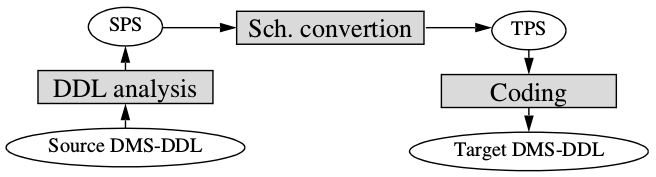
\includegraphics[width=0.9\textwidth]{../images/strategies_fig_02a.png} \\
	\tiny Quelle: \citep{henrard-2002}, Abbildung 2
\end{figure}

Durchf"uhrung auf physischer Ebene sind meist elementare Konvertierungen und m"ussen nicht zwangsweise von Analysten oder fachlich geschultem Personal vorgenommen werden. Die rein physische Konvertierung kann automatisiert durchgef"uhrt werden \citep{abiteboul-1999}.
\lb
Nachteil der physischen Konvertierung ist ein fehlender Mehrwert der entstandenen Daten \citep{henrard-2002}. Vorhandene Schemata werden soweit wie m"oglich auf andere Technologien "ubertragen. Eine fachliche und konzeptuelle Analyse der Daten bleibt aus. In diesem Fall stellt die Migration der Daten lediglich ein Umkopieren in ein neues Datenformat dar.
\lb
Die physische Migration eignet sich vor allem bei einem Wechsel der technischen Umgebung der Daten, etwa einem Wechsel der Version des verwendeten DMS oder einem Wechsel des Herstellers. %TODO Finish

% ===
\subsubsection{Konzeptuell}

Anders als auf physischer Ebene werden Daten auf konzeptueller Ebene auch semantisch betrachtet. Schemata und Datenformate werden evaluiert und neu konzeptioniert. Aus der fachlichen Betrachtung der Daten ergeben sich unter Umst"anden umfangreiche "Anderungen an den Schnittstellen der System. Fachliche Konvertierung erfordern ein Umdenken. Dieses kann die Qualit"at der migrierten Daten verbessern.
\lb
Die konzeptuelle Migration der Daten f"uhrt auf vorhandenen Schemata und Datenformaten eine semantische Analyse durch. Anhand der aus dieser gewonnenen Informationen wird eine Neukonzeptionierung der Modellierung vorgenommen. Abbildung \ref{pic:conversion_conceptual} zeigt das Vorgehen w"ahrend der konzeptuellen Migration. Das Quell-DMS Schema wird mithilfe eines Database Reengineering (BDRE) analysiert \citep{henrard-2002}. Ziel dieses Vorganges ist die Bereinigung (engl.: \textit{Cleansing}) vorhandener Daten \citep{rahm-2010} \citep{hernandez-1998}. Auf Basis einer neuen Konzeptualisierung des der Schemata wird die Konvertierung "ahnlich zur physischen Migration vorgenommen. Neue Formate werden in das Ziel-Format "ubertragen und kodiert. Die Konvertierung und Migration der eigentlichen Daten in die neue Umgebung erfolgt ebenfalls mithilfe von Konvertierungen. Diese ist, im Gegensatz zur physischen Konvertierung, umfangreicher. Neue Abbildungen und Modellierungen m"ussen aus vorhandenen Daten abgeleitet werden.

\begin{figure}[h!]
	\centering
	\caption{Konzeptuelle Konvertierung}
	\label{pic:conversion_conceptual}
	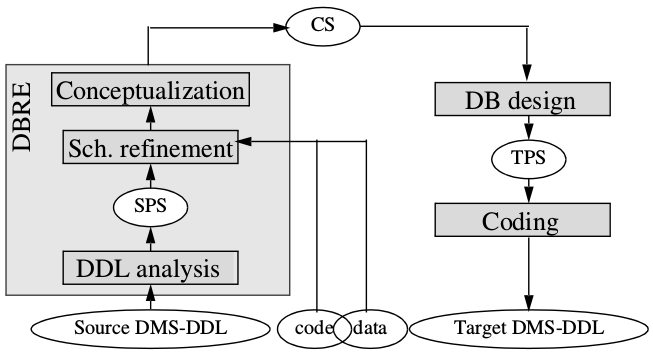
\includegraphics[width=0.9\textwidth]{../images/strategies_fig_02b.png} \\
	\tiny Quelle: \citep{henrard-2002}, Abbildung 2
\end{figure}

Auf konzeptueller Ebene spielt die fachliche Betrachtung vorhandener Daten eine wichtige Rolle. Das Verfahren ist nicht zwangsweise trivial. Analysen und konzeptuelle Konvertierung ben"otigen ein gewisses Verst"andnis der Semantik von Daten.
\lb
Eine konzeptuelle Migration von Daten sorgt vor allem f"ur ein saubere Portierung vorhandener Daten. Schemata werden semantisch korrekt an neue Umgebungen und Formate angepasst. Eine potentielle S"auberung der Daten verringert unter Umst"anden Redundanzen oder nicht ben"otigte Datens"atze oder -formate.
\lb
Der f"ur eine konzeptuelle Migration notwendige Aufwand ist vergleichsweise hoch. Ben"otigte Spezialisten und erforderliches fachliches Verst"andnis von Daten und Umgebung sorgen eventuell f"ur hohe Kosten.
\lb
Fazit %TODO

% ==
\subsection{Anwendungsebene}

Sind Datenformate und Daten selbst konvertiert und migriert, m"ussen umgebende Softwaresysteme angepasst werden. Ver"anderte Datenformate beziehungsweise Technologien setzen oft einen ver"anderten Zugriff auf diese Daten voraus. Um den Aufwand f"ur "Anderung innerhalb der nutzenden Anwendungen m"oglichst zu reduzieren, existieren drei Strategien zu Anpassung von Anwendungen. Die zeichnen sich durch unterschiedliche Ebenen der Anpassung aus. Je nach Tiefe der Anpassung liegen ihnen unterschiedliche Ans"atze zugrunde. 

% ===
\subsubsection{Wrapper}

%TODO Wrapper damit Anwendung auf die Daten wir zuvor zugreifen kann

% ===
\subsubsection{Statements}

%TODO Anpassung der Statements zum Aufruf der Daten 

% ===
\subsubsection{Logik}

%TODO Anpassung der Art und Weise, wie Anwendung Daten und Schemate verwendet